\section{Our Model}

As mentioned in the introduction, we investigate our basic model: segregation of $20$ individuals of type $1$ and $20$ individuals of type $2$ on a $8 \times 8$ board.
In this model an individual moves if less than one third of his/her neighbours is not of his/her type to the nearest place where he/she becomes happier.
Furthermore, the basic model uses the second order neighbourhood: so the maximum number of neighbours is eight.\\

First of all, we can change the size of the board.
Without changing any other parameters, this only implies that the board becomes busier or more quiet.
This results respectively in an increase/decrease of the total number of generations and moves.\\

Secondly, we can also change the number of different types on the board.
For instance, we can look at a $12\times 12$ board with $10$ types of individuals and $10$ individuals per type: see figure \ref{fig:example big board}.
As one can see, far more individuals have been moved to another place on the board and they form groups.

\begin{figure}[H]
	\centering
    \begin{subfigure}{0.45\textwidth}
        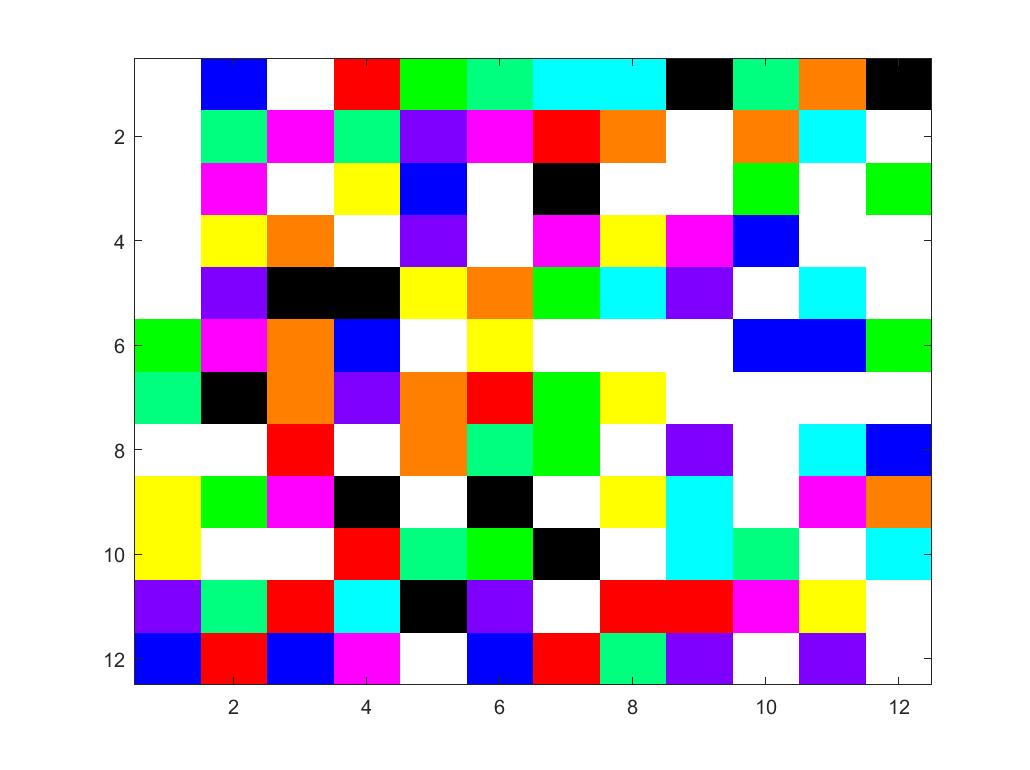
\includegraphics[width=\textwidth]{vb2beginbord.jpg}
        \caption{Situation before segragation}
        \label{fig:example big board begin}
    \end{subfigure}\hspace{0cm}
    ~ %add desired spacing between images, e. g. ~, \quad, \qquad, \hfill etc. 
      %(or a blank line to force the subfigure onto a new line)
    \begin{subfigure}{0.45\textwidth}
        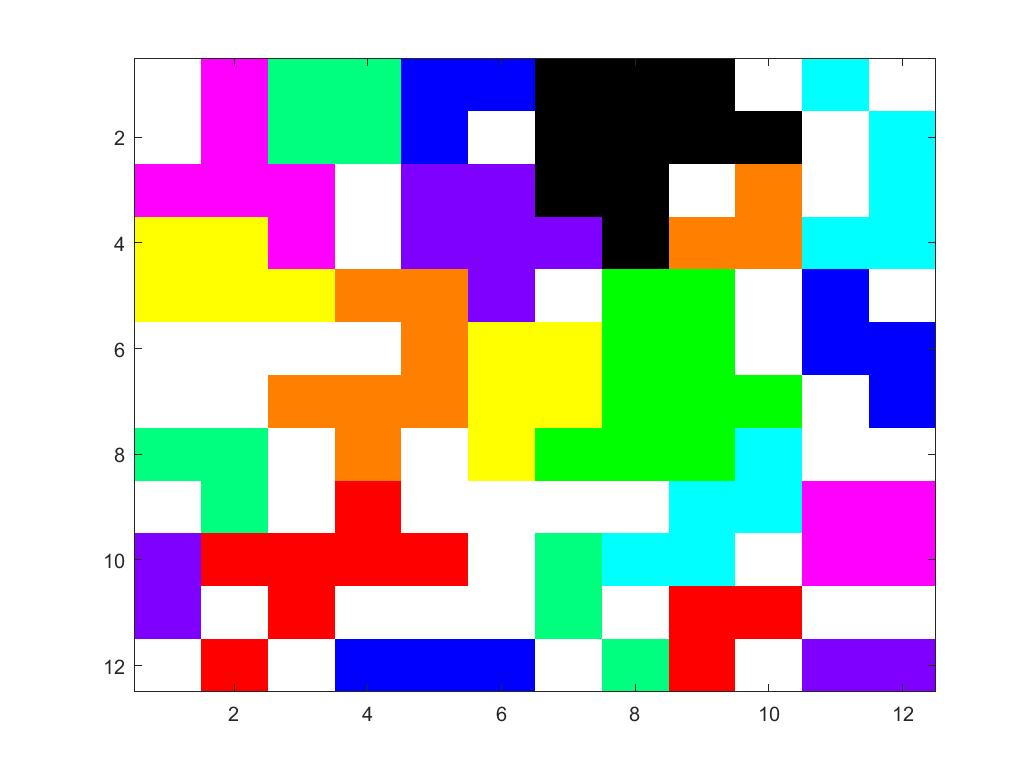
\includegraphics[width=\textwidth]{vb2eindbord.jpg}
        \caption{Situation after segregation}
        \label{fig:example big board end}
    \end{subfigure}
    ~ %add desired spacing between images, e. g. ~, \quad, \qquad, \hfill etc. 
    %(or a blank line to force the subfigure onto a new line)
    \caption{An example of segregation in a model on a $12\times 12$ board with $100$ individual of $10$ different types}
    \label{fig:example big board}
\end{figure}




